\documentclass[aspectratio=169]{beamer}
\usepackage[utf8]{inputenc}
\usepackage{amsmath}
\usepackage{amsfonts}
\usepackage{hyperref}
\usepackage{graphicx}
\usepackage{fontspec}
\usepackage{glossaries}
\usepackage{xcolor}
\usepackage{fontspec}
\usepackage{minted}

\definecolor{cblak}{RGB}{35,35,35} 
\usemintedstyle{solarized-dark}

%\usemintedstyle{tango}

\renewcommand\mathfamilydefault{\rmdefault}
\newcommand{\curdir}{.}


\newfontfamily\Nepali[Scale=1.1,Script=Devanagari]{Laila}
\newcommand{\Devanagari}[1]{{\Nepali #1}}
\newcommand{\code}[2][python]{\mintinline[fontsize=\footnotesize]{#1}|#2|}

\usetheme{CambridgeUS}

\useinnertheme{rectangles}

\input{DarkColour.tex}

%\usefonttheme{professionalfonts} %mkes math fonts original
%\newcommand{\code}[2][python]{\mintinline{#2}|#1|}
\author{Prakash Gautam \\ \Nepali{[ प्रकाश गौतम ]}}
\title{Programming as Physicists}

%\setbeamercovered{transparent}

\date{\today} 
\subject{Physics} 

\begin{document}

\titlepage
%\phantom{\gls{tpc} \gls{roi} \gls{pdf}}\vspace*{-1cm}

%\begin{frame} \frametitle{Outline}
%\tableofcontents
%\end{frame}
\renewcommand{\bf}[1]{\textcolor{red!60}{#1}}

%
%
\section{Jupyter Notebook}
%
\begin{frame}{Jupyter Lab}
    \begin{columns}
        \begin{column}{0.49\textwidth}
            \begin{itemize}
                \item Great tool for prototyping python
                \item Allows interactive sessions, useful while developing code
                \item Can be run in a powerful server, and viewed in local browser (not specific to jupyter only)
            \end{itemize}
            \begin{block}{Caution}
                Don't overuse jupyter notebooks.
            \end{block}
        \end{column}
        \begin{column}{0.49\textwidth}
            
\includegraphics[width=\linewidth]{images/jupyter_logo.png}
        \end{column}
    \end{columns}
\end{frame} 


\begin{frame}[fragile]{Running on Server}
    \begin{itemize}
        \item \code{ssh} tunneling allows accessing web services running on a server.
        \item Since jupyter starts a https web service, we can use ssh to access that
    \end{itemize}
    \begin{minted}[autogobble,fontsize=\scriptsize,bgcolor=cblak,breaklines=true]{bash}
        user@local ~$ ssh username@server
        username@server ~$ cd working/directory
        username@server ~/working/directory $ jupyter lab --no-browser --port=8831
    \end{minted}
    Let this shell running
    \begin{minted}[autogobble,fontsize=\scriptsize,bgcolor=cblak,breaklines=true]{bash}
        user@local ~$ ssh username@server -NL 8831:localhost:8831
    \end{minted}
    Access \url{http://localhost:8831} from local
    \begin{itemize}
        \item End result is accessing remotely running web service in local browser.
    \end{itemize}
\end{frame} 
%
\section{Symbolic Programming}
%
\begin{frame}[fragile]{Sympy}
    \begin{itemize}
        \item Mathematica/Wolframalpha, Maxima, Matlab/Octave Symbolic, 
        \item Python has \code{Sympy}.
            \begin{itemize}
                \item Supports various latex output
                \item Has lot of mathematics and physics library
                \item Extremely useful and easy to use
            \end{itemize}
    \end{itemize}
\end{frame} 
%
%
%
\begin{frame}[fragile]{Cadabra}
     \begin{columns}
        \begin{column}{0.52\textwidth}
            \begin{itemize}
                \item Anybody can appreciate how notorious symbolic tensor analysis are
                \item Sympy has tensor modules, but are not very intuitive to work
                \item Cadabra simply blows my mind
                    \begin{itemize}
                        \item It is very intuitive, minimal 
                        \item Supports almost Latex style input
                        \item Can be used in jupyter notebooks
                    \end{itemize}
            \end{itemize}
            \begin{block}{Cadabra}
                Blows my mind
            \end{block}
        \end{column}
        %
        \begin{column}{0.46\textwidth}
                %\only<1>{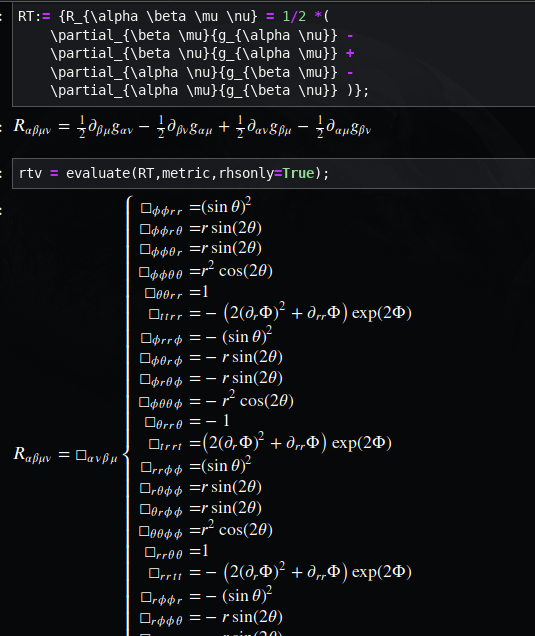
\includegraphics[width=0.78\linewidth]{images/Cadabra2Snap.png}}
                \only<1>{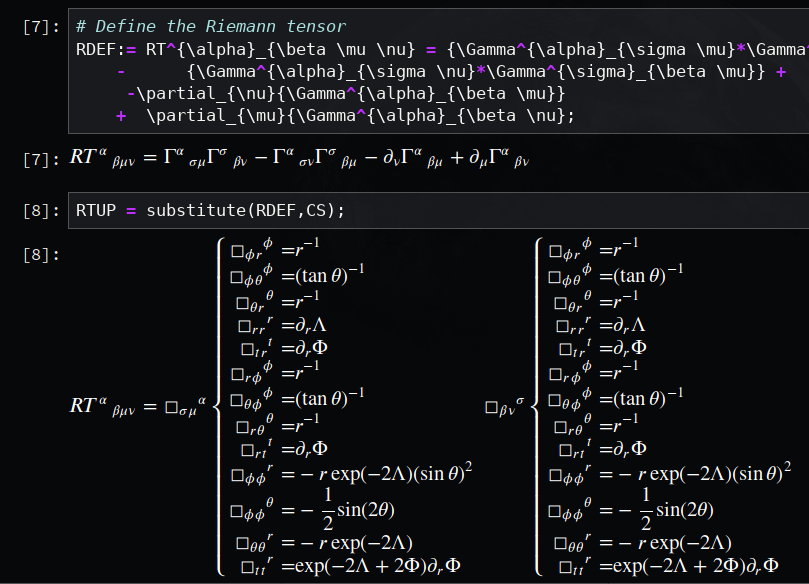
\includegraphics[width=0.88\linewidth]{images/CadabraSnap.png}}
        \end{column}
        %
    \end{columns}
\end{frame} 
%
\section{Programming Paradigm}
%
%
%
%
\begin{frame}[fragile]{Programming Paradigm}
     \begin{columns}
        \begin{column}{0.49\textwidth}
            \begin{itemize}
                \item Modular programming
                \item We write (several) modules/functions to accomplish task
            \end{itemize}
        \end{column}
        \begin{column}{0.49\textwidth}

            \begin{minted}[autogobble,fontsize=\scriptsize,bgcolor=cblak,breaklines=true]{python}
                def histogram(x,bins=10):
                    __ = plt.hist(x,bins=bins)
            \end{minted}
            \begin{minted}[autogobble,fontsize=\scriptsize,bgcolor=cblak,breaklines=true]{python}
                x = np.random.normal(0,1,1000)
                histogram(x,bins=100)
            \end{minted}
        \end{column}
    \end{columns}
\end{frame} 
%
%
\begin{frame}[fragile]{Programming Paradigm}
     \begin{columns}
        \begin{column}{0.39\textwidth}
            \begin{itemize}
                \item Object Oriented Programming (OOP)
            \end{itemize}
        \end{column}
        \begin{column}{0.59\textwidth}

            \begin{minted}[autogobble,fontsize=\scriptsize,bgcolor=cblak,breaklines=true]{python}
                class Histogram():
                    def __init__(self,x,bins=10,weights=None):
                        H,be,bv = np.histogram(x,bins=bins)
                        Hc,be,bv = np.histogram(x,bins=bins,weights=None)
                        self.H = H/Hc
                    def plot(self,ax=None):
                        if ax is None:
                            fig,ax = plt.subplots()

                        ax.plot(self.H,ls='steps')
            \end{minted}

            \begin{minted}[autogobble,fontsize=\scriptsize,bgcolor=cblak,breaklines=true]{python}
                x = np.random.normal(0,1,1000)
                h = Histogram(x,bins=100)
                h.plot()
            \end{minted}
        \end{column}
    \end{columns}
\end{frame} 
%
%
%\titlepage
%
%
\begin{frame}[fragile]{Make Distributable Code}
    \begin{itemize}
        \item Assume other people are going to use your code.
        \item Portable code is better maintainable.
        \item It is lot more extensible. (From my painful experience)
    \end{itemize}
\end{frame} 
%
%
%
%
\begin{frame}[fragile]{Python Packages}
    \begin{columns}
        \begin{column}{0.52\textwidth}
            \begin{itemize}
                \item Python modular hierarchy
                    \begin{itemize}
                        \item Statements/Expression
                        \item functions/Modules
                        \item Class
                        \item package
                        \item Library
                    \end{itemize}
                \item An (possibly emmpty) \code{___init__.py} tells python that it is a package
                \item Python looks for library/package in \code{PYTHONPATH} environment variable\\
            \begin{minted}[autogobble,fontsize=\scriptsize,bgcolor=cblak,breaklines=true]{bash}
                export PYTHONPATH=package/location:$PYTHONPATH
            \end{minted}

            \end{itemize}
        \end{column}
        \begin{column}{0.46\textwidth}
            \only<1>{\inputminted[fontsize=\large,bgcolor=cblak]{text}{./package_hier.txt}}
        \end{column}
    \end{columns}
\end{frame} 
\begin{frame}{Matplotlib styling}
    \begin{columns}
        \begin{column}{0.58\textwidth}
            \begin{itemize}
                \item We can use style files to customize plots
                \item Comes handy when we need different version of same plot
                \item Requires no modification in code
                \item \code{~/.config/matplotlib/stylelib/mystyle.mplstyle} file
                \item In the code use \code{plt.style.use("mystyle")}
            \end{itemize}
        \end{column}
        \begin{column}{0.40\textwidth}
                \only<1>{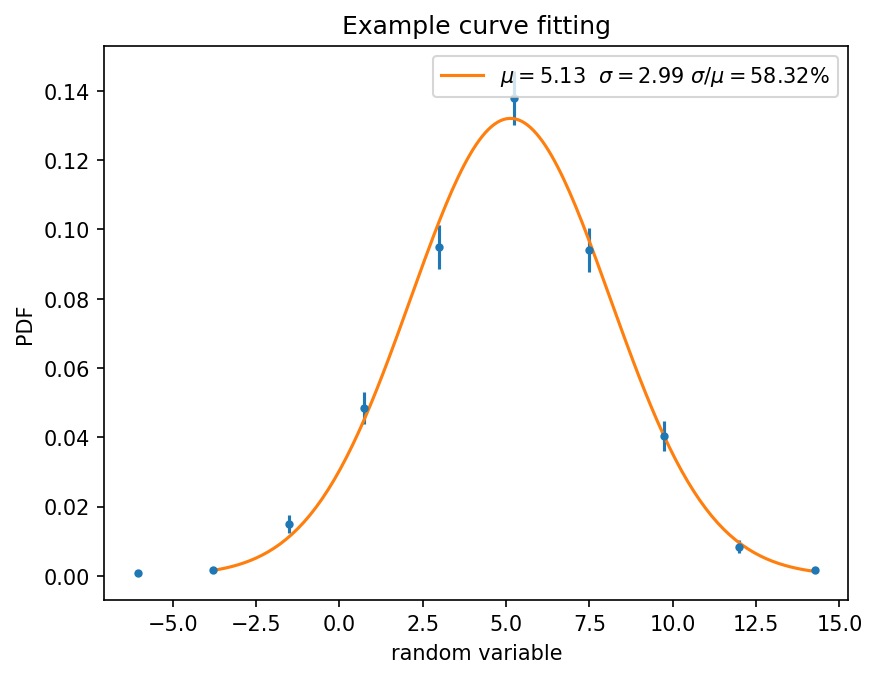
\includegraphics[width=0.88\linewidth]{images/demo_fit_light.png}}
                \only<2>{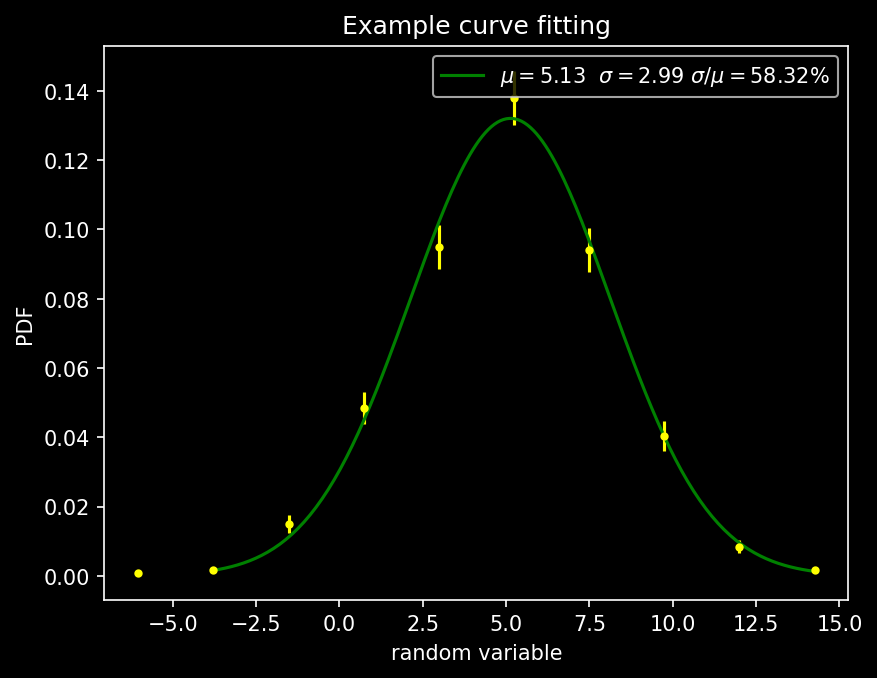
\includegraphics[width=0.88\linewidth]{images/demo_fit_default.png}}
                \only<3>{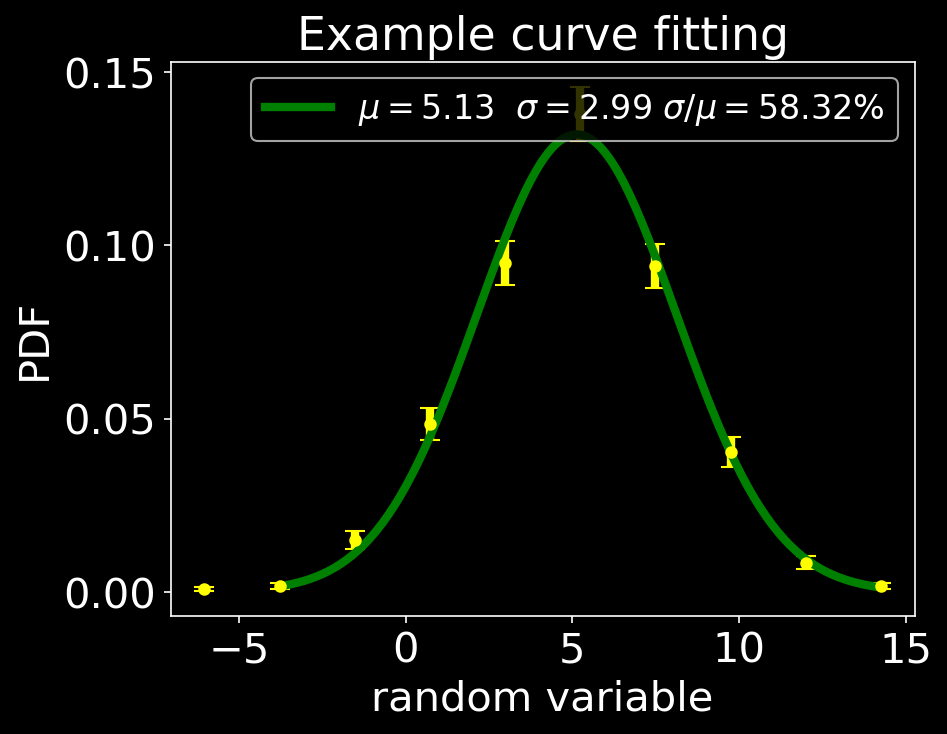
\includegraphics[width=0.88\linewidth]{images/demo_fit_slide.png}}
                \only<4>{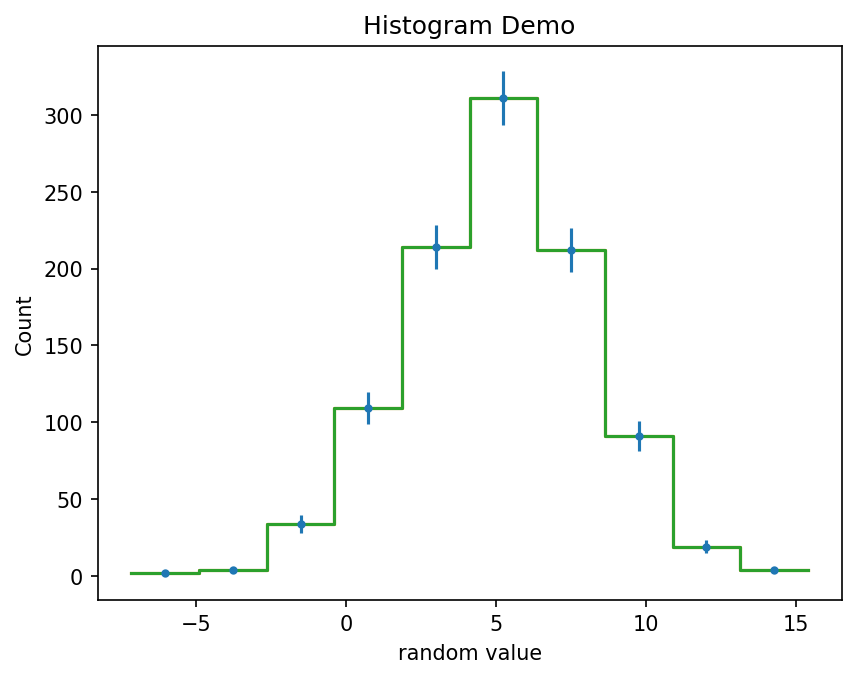
\includegraphics[width=0.88\linewidth]{images/demo_hist_light.png}}
                \only<5>{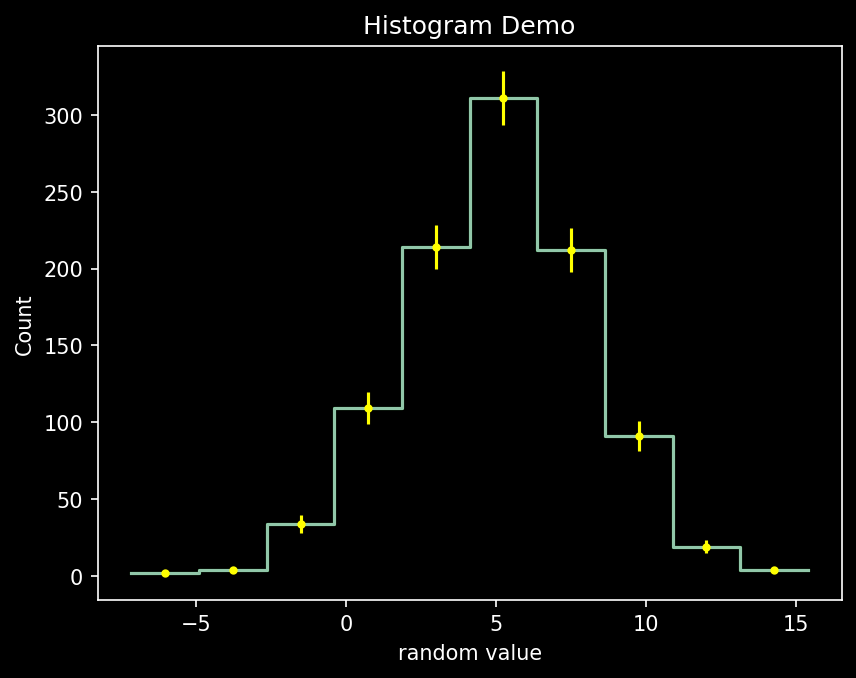
\includegraphics[width=0.88\linewidth]{images/demo_hist_default.png}}
                \only<6>{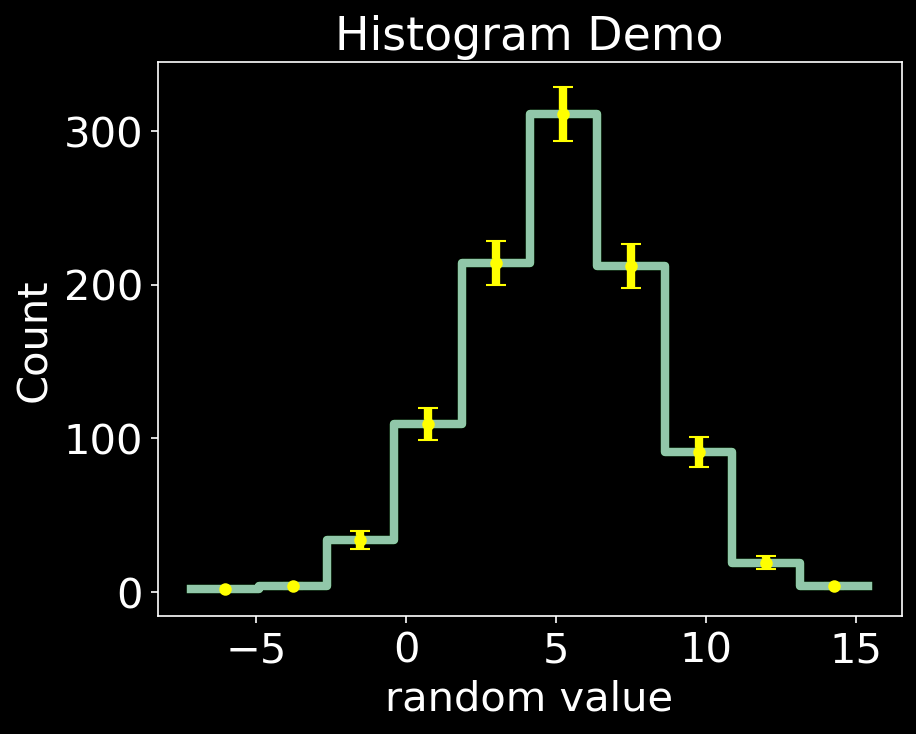
\includegraphics[width=0.88\linewidth]{images/demo_hist_slide.png}}
        \end{column}
    \end{columns}
\end{frame} 


%
\end{document}

